\documentclass{article}

% if you need to pass options to natbib, use, e.g.:
%     \PassOptionsToPackage{numbers, compress}{natbib}
% before loading neurips_2020

% ready for submission
% \usepackage{neurips_2020}

% to compile a preprint version, e.g., for submission to arXiv, add add the
% [preprint] option:
%     \usepackage[preprint]{neurips_2020}

% to compile a camera-ready version, add the [final] option, e.g.:
     \usepackage[preprint,nonatbib]{neurips_2020}

% to avoid loading the natbib package, add option nonatbib:
    % \usepackage[nonatbib]{neurips_2020}

\usepackage[utf8]{inputenc} % allow utf-8 input
\usepackage[T1]{fontenc}    % use 8-bit T1 fonts
\usepackage{hyperref}       % hyperlinks
\usepackage{url}            % simple URL typesetting
\usepackage{booktabs}       % professional-quality tables
\usepackage{amsfonts}       % blackboard math symbols
\usepackage{nicefrac}       % compact symbols for 1/2, etc.
\usepackage{microtype} 
\usepackage{amsmath}     % microtypography
\usepackage{rotating}
\usepackage{graphicx}
\graphicspath{ {../images/} }

\usepackage[backend=bibtex]{biblatex}
\addbibresource{biblio.tex}

\DeclareMathOperator*{\argmin}{arg\!\min}

\title{An Introduction to Machine Learning Methods and Email Spam Filtering}

% The \author macro works with any number of authors. There are two commands
% used to separate the names and addresses of multiple authors: \And and \AND.
%
% Using \And between authors leaves it to LaTeX to determine where to break the
% lines. Using \AND forces a line break at that point. So, if LaTeX puts 3 of 4
% authors names on the first line, and the last on the second line, try using
% \AND instead of \And before the third author name.

\author{%
 Justin Hiemstra \\
  Department of Electrical and Computer Engineering\\
  University of Wisconsin, Madison\\
  Madison, Wi. 53704 \\
  \texttt{justinhiemstra@protonmail.com} \\
  % examples of more authors
  % \And
  % Coauthor \\
  % Affiliation \\
  % Address \\
  % \texttt{email} \\
  % \AND
  % Coauthor \\
  % Affiliation \\
  % Address \\
  % \texttt{email} \\
  % \And
  % Coauthor \\
  % Affiliation \\
  % Address \\
  % \texttt{email} \\
  % \And
  % Coauthor \\
  % Affiliation \\
  % Address \\
  % \texttt{email} \\
}

\begin{document}

\maketitle

\section{Code}
All code for this project, along with other text files, and generated images can be found on GitHub at
\section{Introduction}
In 1971, when for the first time computer engineer Ray Tomlinson used a computer to send a text message containing the @ symbol as a part of its address to another location within the ARPANET, the communication technologies of yesteryear like the bulletin board saw the writing on the wall -- their time to enter the annals of obscolecence had come.  And in the almost 50 years since the transmission of the first email, emails have truly transformed the way people communicate at every level of society, from academia to the professional workplace, from interpersonal relations to mass media advertising. But as is often the case with any new revolutionary new technology that has tremendous promise to make the world a better place, there exists a subset of people who would rather see that technology twisted for their own purposes, be they malice or profit. For emails, this takes the form of the dreaded spam email, which can be used to convey things such as malware, or to advertise unwanted products. By the mid-1990s, spam email had become sufficiently problematic that academics started exploring ways to apply filters that would prevent these emails from entering an email user's inbox. Early attempts performed quite poorly, as they were based on "keyword" filters that would block emails containing any of a subset of flagged words. While this resulted in a good number of spam emails being blocked, it also had the ill effect of placing a user's legitimate emails in the trash, and because for most people the prospect of not receiving a legitimate email is magnitudes of order worse than finding a spam email in their inbox, this was highly undesirable\cite{Livingston2002}. Thankfully, this topic has progressed tremendously, and modern adaptive email spam filters based heavily on machine learning (ML), such as those deployed by Google, are able to correctly classify over 99.9\% of all emails with a false positive rate (ie the rate at which legitimate emails are accidentally labeled as spam) of less than 0.05\%\cite{Metz2015}.

This paper is an introductory exploration of the efficacy of several topics covered in ECE 532 -- Matrix Methods in Machine Learning as they are applied to the task of spam email filtering. Specifically, least-squares regression, kernelized support vector machines, and neural networks have been implemented and trained using a test dataset of "ham" (legitimate emails, ie anything that isn't spam) and spam emails. One additional method not covered in class, a Naive Bayesian Inference filter, has also been implemented because it was this type of filter that was the first to obtain a notable level of success.

\section{Methodology}
The first task in implementing any of these ML topics is to have workable data. Because emails are text-based and all of these methods must take as input some form of numerical data, any set of training data must first be turned into numbers to be passed to the models. Several methods for this exist, but this paper will use the basic \emph{Bag-of-Words model}. To understand the premise of this model, considering the following text:

\begin{center}
\texttt{The dog named James walked down the street.}
\end{center}

The first step of implementing Bag-of-words is defining a dictionary, which for the dataset used later in this paper will be done by looking at every word that occurs within the dataset. In this example text, there are 8 words, 7 of which are unique. Before placing these words in the dictionary, they are standardized by making everything lowercase and stripping punctuation. Thus, the dictionary, $D$, for this text becomes

\begin{center}
$D = (\texttt{"the", "dog", "named", "james", "walked", "down", "street"})$
\end{center}

With an ordered dictionary, each set of text (ie the emails) is turned into a vector, where every entry of the vector corresponds to the number of times that indexed word appears in the text (some Bag-of-Words models do not consider the frequency with which a word occurs in the text, but the model used in this paper does because it should theoretically give more information about the contents of each email). In the case of the example text with the ordered dictionary $D$, this vector is just

\begin{center}
$x = [2,1,1,1,1,1,1].$
\end{center}

Note that this model does not encode a significant amount of information about each text. It loses any concept of grammar, formatting of text, and ordering of words. Despite these deficiencies, it is a commonly used approach, as many spam filters make the assumption that it is the words themselves that give information about whether an email can be correctly identified as ham or spam, and based on the results of some ML implementations in this paper, this assumption must be at least somewhat valid.


With a set of emails that have been classified as either ham or spam, a data matrix can be built by first building a dictionary based on the words occurring in those emails, and then finding the corresponding vectors for those emails. This matrix has rows that correspond to each individual email, and columns that correspond to the number times a given word from the dictionary appears in that email. Once the email dataset has been turned into a bag of words, the ML topics mentioned earlier can be effectively applied to build classification models.



\section{Implementation and Results}
\subsection{Dataset Used}
The dataset used in this paper, which can be found at \url{http://nlp.cs.aueb.gr/software_and_datasets/Enron-Spam/},  is a classic email dataset that was compiled from emails received by employees at the now defunct energy company Enron. Within the dataset, there are 3672 ham emails and 1500 spam emails for a total of 5,172 emails, all received between 1999-12-10 and 2005-09-06. Emails are unedited and in their "raw" form, although they do not contain any email headers. As a sample, this is one spam email from the dataset:


\begin{figure}[h]
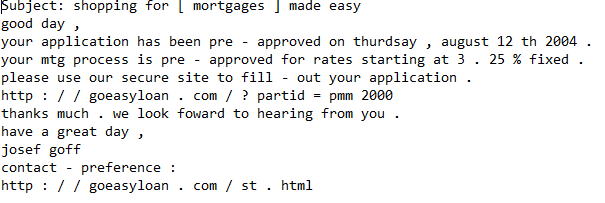
\includegraphics[scale=0.75]{spam_example.PNG}
\caption{Example spam message from Enron dataset}
\centering
\end{figure}

Within the dataset, emails are kept as .txt files and assigned names based on their ordering within the dataset, the date they were received, who received them, and whether or not they were labeled by hand as ham or spam. An example file name is \texttt{0001.1999-12-10.farmer.ham.txt}.


\subsection{Data Preprocessing}
Some preprocessing of this data was first necessary. To implement the Bag-of-words model in Python, a dictionary was first created by iterating through each email and adding any new words to a list. Once again, all punctuation was stripped and all words were first made lowercase. It should be noted that some of the emails were modified to make this process easier, because several of the spam emails contained punctuation that was not encoded in UTF-8. These emails threw errors in python because they were not readable, and as a workaround, the non-UTF punctuation in those emails was first found and stripped. Because punctuation is not considered in the bag-of-words model, these alterations should have no affect on the overall legitimacy of the data.

Once the dictionary was created, a data matrix was built by iterating through each email and finding its associated bag-of-words vector. A vector containing labels/classifications for each email was then created by determining whether each email name contained the phrase "ham" or "spam." Ham emails were assigned the value $1$, and spam emails were assigned a value of $-1$.

One thing to note is that each email in the dataset begins with the word \texttt{Subject}. This word was included in the dictionary with its first letter capitalized as it appeared in the emails, because it effectively acted like a built in all-1s vector that is often added to data for the purpose of translation when implementing things like least-squares. With the inclusion of this word, the final dictionary contained $45,849$ unique entries. Furthermore, the dictionary was compiled using the entire dataset, although things like cross-validation were used. This was to ensure that any word appearing in a given email would be present in the dictionary. 



\subsection{Least-squares Implementation Results}
The first classifcation model that was implemented was least-squares regression. From the outset, it was assumed that this model would perform poorly given the high-dimensional nature of the featurespace for the data, coupled with the relative sparcity of each email's word vector. The least-squares regression implementation for this paper was coded entirely from scratch without the use of any pre-existing Python packages. In general, least-squares regression involves finding a solution 
$$\hat{w} = \argmin_w{ ||y-Aw||^2_2}$$ where $y$ is the vector containing classifications, $A$ is the matrix of training data, and $w$ is a vector of weights indicating the importance of each feature as it pertains to classification (when features are referred to in the context of this paper, they represent the words contained in the dictionary). The solution to this is generally found as $$\hat{w} = (A^TA)^{-1}A^Ty$$ although because of the complexity of inverting a high-dimensional matrix, an identity was used to find $$\hat{w} = A^T(AA^T)^{-1}y.$$ This calculation assumes the invertability of $AA^T$, which requries that $A$ be full-rank. However, in the case of the data matrix for the Enron dataset, this was not the case because many spam emails appeared multiple times. To fix this problem, a modified dataset was first computed by removing any duplicate emails.

 Although in general least-squares regression need not be linear, linear least-squares was implemented here for the sake of not making any larger an already $45,849$-dimensional featurespace.

This classification model was assumed to have a relatively low chance of correctly labeling any significant amount of emails because of the sparcity of the data matrix, the high-dimensional featurespace, and the linearity of the model. Unsurprisingly, it performed quite poorly with a misclassification rate of 42.11\%, or of the modified dataset $1932$ misclassifications. To understand whether this misclassification rate is truly any better than a model that just randomly guesses whether a given email is ham or spam based on the distribution of ham/spam emails, consider the underlying probabilistic distribution that would govern such an event: because randomly assigning a classification to given email is a Bernoulli event (in the case of the Enron dataset, the likelihood of "success," or an email being ham is about $0.68$), then the likelihood of assigning classifications to $N = 5172$ emails is governed by the probability mass function of the Binomial distribution with $p = 0.68$, $N = 5172$, and $K = \texttt{\# of emails correctly classified}$. With this information, the Binomial distribution cumulative density function can be used to gain some insight into the likelihood that a guessing model could outperform the linear least-squares model. Notably, it was found that the likelihood of outperforming the linear least-squares model was about .46, indicating that this model performs quite poorly. Because of how poorly the model performed, cross-validation techniques were not implemented, because the model trained on the entire modified dataset was barely better than guessing, and cross-validation techniques are primarily employed to assess whether or not a model has been over-fit to its training data. This was clearly not the case.


\subsection{Kernelized SVM Implementation Results}
The second classification model that was implemented in Python (this time against the full dataset, not the modified least-squares dataset) was a kernelized support vector machine (SVM). Rather than building the mechanics of the SVM from scratch, a pre-existing Python library from Scikit-Learn was used. Notably, there are two libraries from Scikit-Learn that implement slightly different SVMs. The first library implements the classic SVM, and takes as inputs things like which kernel to use, how large the regularization term should be to prevent over-fitting, how many iterations of stochastic gradient descent (SGD) to perform, and in the case of a polynomial kernel, the degree of the used polynomial. For whatever reason this implementation failed quite miserably -- it never caught any spam, leading to a false negative rate of 100\% --  regardless of the input parameters given. The second library, called \texttt{NuSVM}, differs from the standard library in that it can also take an argument to define the number of support vectors to use. Thankfully, \texttt{NuSVM} did perform rather well. Because parameter selection is very important for these types of models, multiple models with different parameters were trained using a random subset consisting of two thirds of the full training data, and then their efficacy was tested against the remaining dataset not used in training. Some of the results for testing each parameterized model on a holdout set of 1724 emails is provided in the following table:

\begin{table}[h!]
\begin{center}
\caption{Parameterized Kernelized SVM Results}
\hspace*{-1cm}\begin{tabular}{c|c|c|c|c}
\textbf{Kernel} & \textbf{Regularization Parameter} & \textbf{Polynomial Degree}& \textbf{Misclassification Rate} \\
\hline
\textbf{Polynomial} &   $1e^{-5}$   &   6 &  24.44\%  \\
\textbf{Gaussian} & $1e^{-4}$  & -- & 6.79\%   \\
\textbf{Gaussian} & $1e^{-3}$  & -- & 6.79\%   \\
\textbf{Gaussian} & $1e^{-6}$  & -- & 6.79\%   \\
\textbf{Sigmoid} & $1e^{-5}$  & -- & 9.40\%   \\
\end{tabular}
\end{center}
\end{table}

As can be seen from the table, the Gaussian-kernelized SVMs had the lowest misclassification rate, and they were interestingly invariant under the regularization term, indicating that some convergence had taken place and that over-fitting was not a concern. These models were additionally run against several different random subsets of data, and the results of each run were similar. 

Because the \emph{types} of misclassifications are also important (such as ham incorrectly labeled as spam, a false positive, and spam incorrectly labeled as ham, a false negative), the following table shows what types of misclassifications are being made by these various models (some of the parameters have been dropped for the sake of brevity in the table):

\begin{table}[h!]
\begin{center}
\caption{Parameterized Neural Nets}
\hspace*{-1cm}\begin{tabular}{c|c|c}
\textbf{Kernel} & \textbf{False Positive Rate} & \textbf{False Negative Rate}\\
\hline
\textbf{Polynomial} &  0\% &  100\%  \\
\textbf{Gaussian} &  67.52\% &  32.48\%  \\
\textbf{Sigmoid} &  21.61\% &  78.39\%  \\
\end{tabular}
\end{center}
\end{table}
These results are particularly interesting, because while the Gaussian kernel has the lowest overall misclassification rate, it also has a proportionally higher false positive rate. Because this is highly undesirable (a very low false positive and a high false negative rate is preferred). Despite the Sigmoid kernel doing a worse job with classification, it has a more ideal ratio of false positives to false negatives.

Overall, the kernelized SVMs are clearly capturing some underlying conditions about the nature of spam and ham emails, as evidenced by these low misclassification rates. This shows that enough information remains encoded in the Bag-of-Words model to at least partially model the data.

\subsection{Neural Networks Implementation Results}
The third classification model that was implemented was Neural Networks. Once again, pre-existing Python packages were used to avoid building the rather complicated neural networks from scratch (this would require significantly more work than even the kernelized SVMs). The package used for this came from Scikit-Learn and is called the \texttt{MLPClassifier}. It takes several things as inputs, including but not limited to the number of hidden layers to use, how many nodes exist at each layer, the activation function to use, a regularization parameter, and the number of iterations/epochs to perform for SGD. Again, many models with different parameter selection were run in an effort to find which parameter values yielded the best results. The following table includes classification results for some of the models as they were tested on a holdout dataset of 1724 emails\footnote{Notice that the activation function used for each instance in the table is the Rectified Linear Unit. This is because using the logistic sigmoid activation function with this Python package failed in every instance regardless of parameter selection, labeling every email as ham. Any future implementation of neural nets may wish to switch to other Python packages like PyTorch, as this is most likely the result of bad code within the Scikit-Learn library.}:


\begin{table}[h!]
\begin{center}
\caption{Parameterized Neural Network Results}
\hspace*{-1cm}\begin{tabular}{c|c|c|c|c}
\textbf{Activation Function} & \textbf{Hidden Layers} & \textbf{Nodes at each Layer} & \textbf{Regularization} & \textbf{Misclassification Rate}\\
\hline
\textbf{ReLU} & 2 &3,3 &$1e^{-3}$ & 2.32\% \\
\textbf{ReLU} & 2 &5,2 &$1e^{-3}$ & 1.80\% \\
\textbf{ReLU} & 3 &3,3,3 &$1e^{-3}$ & 2.26\% \\
\textbf{ReLU} & 3 &5,3,2 &$1e^{-3}$ & 1.91\% \\
\textbf{ReLU} & 5 &3,3,3,3,3 &$1e^{-3}$ & 2.84\% \\
\textbf{ReLU} & 4 &5,4,3,2 &$1e^{-3}$ & 1.57\% \\
\textbf{ReLU} & 4 &5,4,3,2 &$1e^{-4}$ & 1.83\% \\
\textbf{ReLU} & 4 &5,4,3,2 &$1e^{-2}$ & 2.03\% \\
\textbf{ReLU} & 4 &5,4,3,2 &$1e^{-1}$ & 2.24\% \\
\textbf{ReLU} & 4 &5,4,3,2 &$1$ & 2.44\% \\
\textbf{ReLU} & 7 &10 at each &$1e^{-4}$ & 28.02\% \\
\end{tabular}
\end{center}
\end{table}

As can be seen, the neural networks performed quite nicely, the best of which had a misclassification rate of only 1.57\%. This extraordinary given the simplistic Bag-of-Words model that was used. A few more interesting things to see in the table include the evidence of overfitting, which can be seen in the case of 7 hidden layers with 5 nodes each. When this model was run against the training data, it correctly labeled 100\% of the emails, but it did not extrapolate well to new data. Another point worth noting is that a descending approach to layer nodes also seems to perform better. 

Once again, it is also useful to view the types of misclassifications that were made. The following table provides misclassification types for a select few neural networks that appear to be fairly representative of the rest:
\newpage
\begin{table}[h!]
\begin{center}
\caption{Parameterized Neural Network Results}
\hspace*{-1cm}\begin{tabular}{c|c|c|c|c}
 \textbf{Hidden Layers} & \textbf{Nodes at each Layer} & \textbf{Regularization} & \textbf{False Positive Rate} & \textbf{False Negative Rate}\\
\hline
 2 &3,3 &$1e^{-3}$ & 37.5\% & 62.5\%\\
 2 &5,2 &$1e^{-3}$ & 67.7\% & 32.3\%\\
 3 &3,3,3 &$1e^{-3}$ & 38.5\% & 61.5\%\\
 3 &5,3,2&$1e^{-3}$ & 63.6\% & 36.4\%\\
 4 &5,4,3,2 &$1e^{-3}$ & 85.2\% & 14.8\%\\
\end{tabular}
\end{center}
\end{table}

As with the kernelized SVMs, there is a tradeoff between overall misclassification performance and the types of misclassifications that are made, with the neural nets containing the same number of nodes at each hidden layer making more misclassifications, but fewer of the undesirable false positives. Despite these neural nets making more misclassifications, they may actually be a more desirable model because they are very accurate, but they make fewer false positives.

Overall, these neural networks were the best performers of all the models that were approached to filter spam in this paper.

\subsection{Naive Bayesian Inference Filter Implementation and Results}
The final model that was implemented for spam filtering was a Naive Bayes filter. Because this topic was not covered in class, and because the 5-page limit has already been surpassed, an in-depth explanation of these filters will not be discussed here\footnote{If you're interested in this topic, you can learn more by visiting \cite{Heckerman1998}. The Wikipedia page is also quite informative}. However, the basic model relies on probability theory and  Bayes' Theorem, which describes conditional probability and is stated as follows\cite{Heckerman1998}:
$$P(S|W) = \frac{P(W|S)P(S)}{P(W)}$$
 In this case, we think of $S$ as spam and $W$ is a word. It makes the assumption that the likelihood of any word appearing is independent of the presence of other words, which is clearly not true for natural language (hence why it is called a "Naive" filter), but this simplification allows easy computation and still yields decent results. The actual implementation of the spam filter uses an equation derived from Bayes' Theorem and the law of Total Probability\cite{Heckerman1998}:
$$P(S|W) = \frac{P(W|S)P(S)}{P(W|S)P(S) + P(W|H)P(H)}$$
where $H$ designates ham email.

The implementation of the Naive Bayes Filter yielded results that were much poorer than those of modern ML approaches (SVMs and Neural Nets), but are still respectable considering the simplicity of the approach. The misclassification rate when run against a holdout set of data of 1724 emails was between 12 and 16 percent, with around a 3:1 false positive to false negative misclassification rate.

\section*{Conclusion}
Unsurprisingly, the spam filters implemented by major email providers like Google far, far exceed what was obtained in this paper. This is due in part because of the vast amounts of data these companies have, the tremendous amount of computational power they possess, and their reliance on the most cutting edge research in spam filtering. Even so, the neural networks implemented worked quite surprisingly well despite using a very simple Bag-of-Words model as input. As to the applicability of these models on emails outside the dataset, the answer is uncertain. Certainly the types of spam emails that are sent have evolved over the years, and it is plausible that the spam in the Enron dataset do not look like modern-day spam. Coupled with the relatively small amount of data (5000 emails is but a drop in the ocean of what is sent on a daily basis), it is very likely that these models would perform extremely poorly were they to be implemented on emails sent today. Nevertheless, the principles used in creating these models, given enough data and enough computation power, could easily be trained on modern datasets and would likely perform nearly as well as they did in these examples.



\newpage
\printbibliography

\end{document}
